\chapter{Rough calculations}
One way to verify the results of your finite element analysis is to compare them with analytical solutions when available. Sometimes there is no analytical solution for the problem at hand, but you can use some approximation that can give us a clue about the accuracy of your analysis. This chapter describes the routines in the \href{https://github.com/xcfem/xc/tree/master/python_modules/rough_calculations}{\tt rough\_calculations} package, that are written for that purpose. 

\section{Punching shear}
\begin{verbatim}
import rough_calculations.ng_punzonamiento as punch
\end{verbatim}
\begin{center}
\begin{tabular}{p{3cm}p{9.5cm}}
\multicolumn{2}{l}{{\tt punch.esfuerzoPunzonamiento(qk,A)}} \\
& rough estimation of the load on the slab over a support \emph{(HL.3 num. gordos)}\\
\multicolumn{2}{l}{{\tt punch.punzMaximo(fck,d,a,b)}} \\
& rough estimation of the maximum punching force with no need of reinforcement for punching shear  \emph{(HL.3 num. gordos)}\\
\multicolumn{2}{l}{{\tt punch.reinforcementPunz(Vd,fck,d,a,b,h,fyd)}} \\
& rough estimation of the reinforcement for punching shear  \emph{(HL.3 num. gordos)} \\
\end{tabular}
\end{center}

where:
\begin{paramFuncTable}
\qkSlab{} \\
\ASupport{} \\
\fck{}\\
\dEff{of the slab} \\
\abSupport{} \\
\h{of the slab} \\
\fyd{of the reinforcement steel} \\
\end{paramFuncTable}

\subsection{Beam deflections}
\begin{verbatim}
import rough_calculations.flechas_vigas as beamDefl
\end{verbatim}
\begin{center}
\begin{tabular}{p{3cm}p{9.5cm}}
\multicolumn{2}{l}{{\tt beamDefl.deflCantBeamPconcentr(l,EI,P,a)}} \\
& maximum deflection in a cantilever beam with a concentrated load at any point \\
\multicolumn{2}{l}{{\tt beamDefl.deflCantBeamQunif(l,EI,q)}} \\
& maximum deflection in a cantilever beam with a uniformly distributed load\\
\multicolumn{2}{l}{{\tt beamDefl.deflCantBeamMend(l,EI,M)}} \\
& maximum deflection in a cantilever beam with a couple moment at the free end\\
\multicolumn{2}{l}{{\tt beamDefl.deflSimplSupBeamPconcentr(l,EI,P,b)}} \\
& maximum deflection in a  beam simply supported at ends with a concentrated load at any point\\
\multicolumn{2}{l}{{\tt beamDefl.deflSimplSupBeamQunif(l,EI,q)}} \\
& maximum deflection in a beam simply supported at ends with a uniformly distributed load\\
\multicolumn{2}{l}{{\tt beamDefl.deflSimplSupBeamMend(l,EI,M)}} \\
& maximum deflection in a beam simply supported at ends with a couple moment at the right end\\
\end{tabular}
\end{center}

\begin{paramFuncTable}
\lSpan{} \\
\EI{} \\
\Pload{} \\
\qload{} \\
\Mcoup{} \\
a & distance from the left end of the beam \\
b & distance from the right end of the beam \\
\end{paramFuncTable}

\clearpage
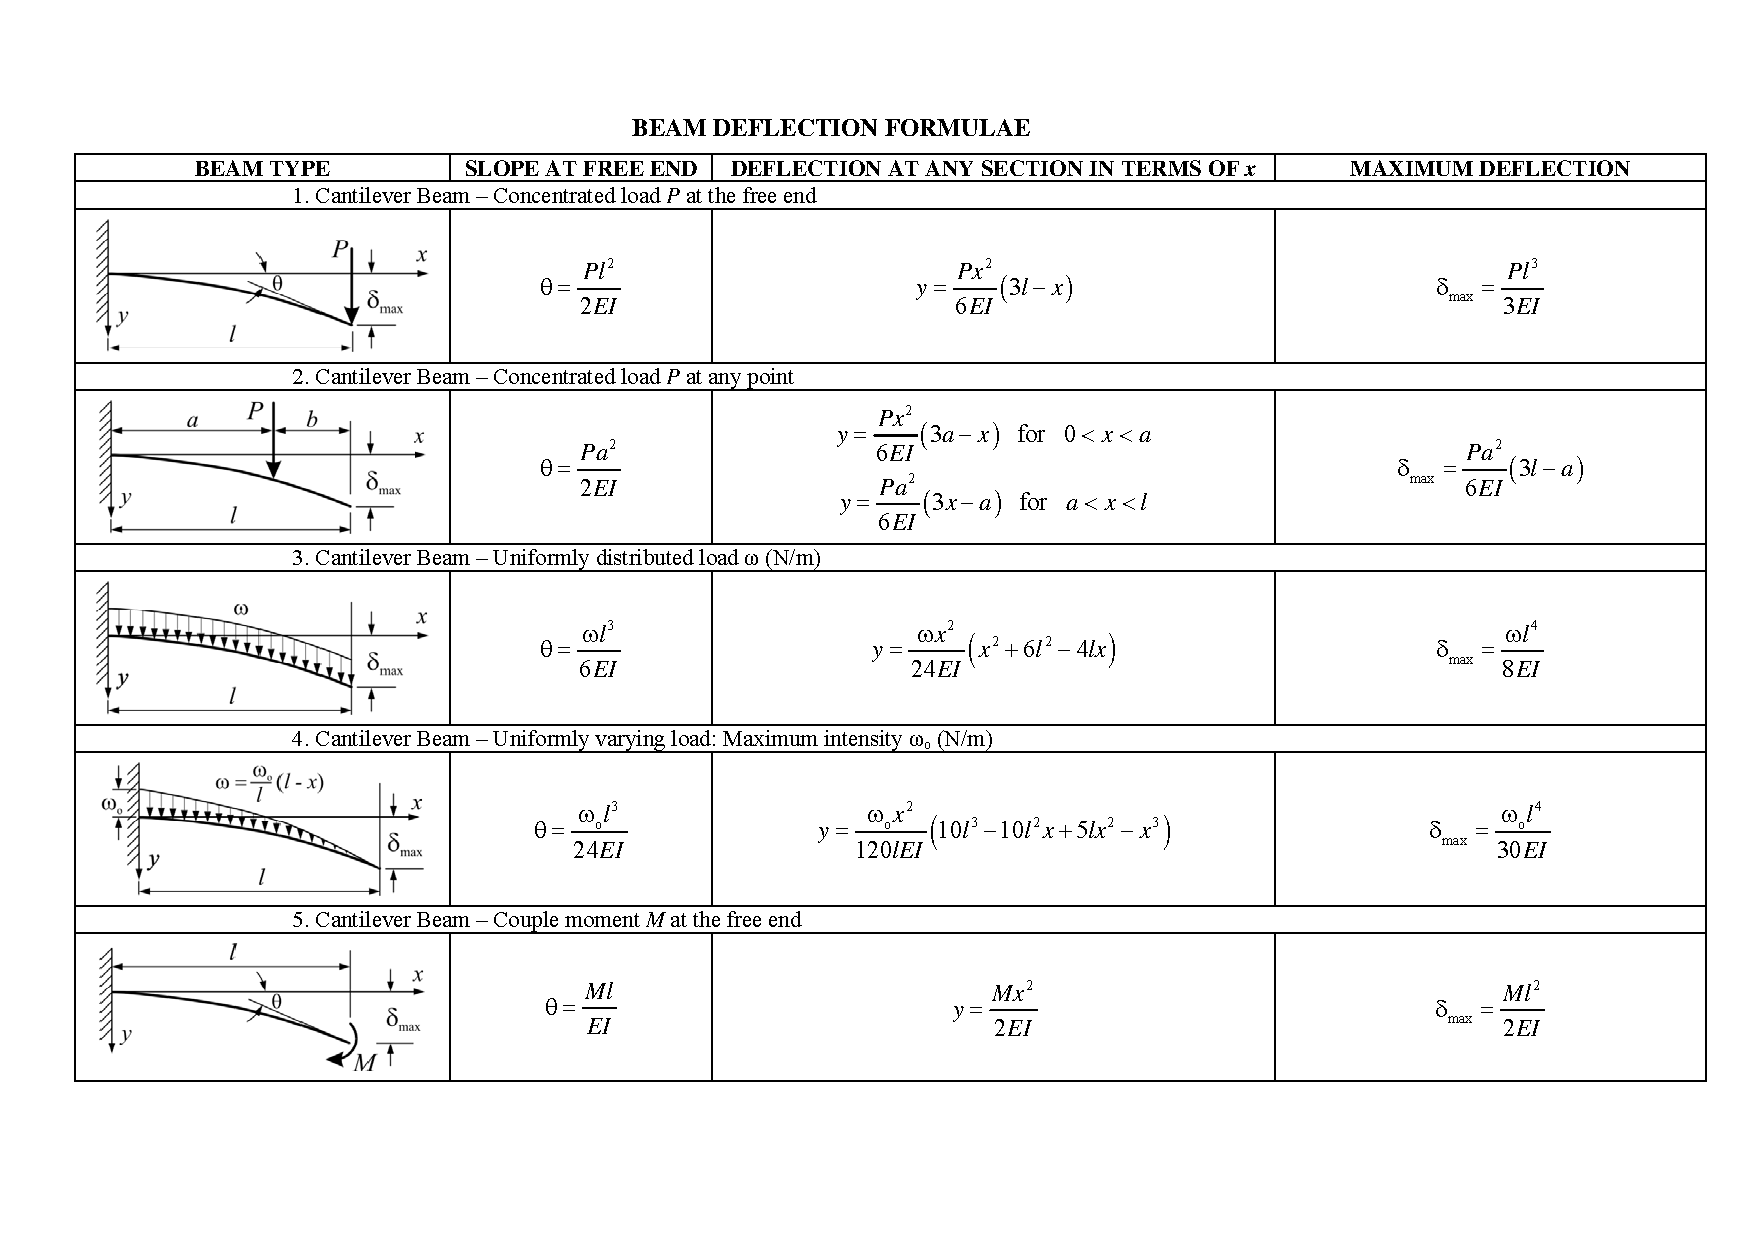
\includepdf[pages={1-2}]{appendix/rough_calculations/figures/beam_formulas.pdf}

\section{Masonry bridge}
Functions for the assessment of a masonry arch bridge by means of a deterministic analytical method.

In these routines, the mechanism method programmed is used for a single-span masonry in a limit analysis, giving a load carrying capacity and a failure mode of the structure. The algorithm of the method applies the kinematic approach. It uses the assumption that a masonry arch becomes a mechanism when at least four plastic hinges appears in the arch barrel. A strict and efficient calculation for unknown position of hinges is based on application of a linear programming algorithm with a target function minimising a live load factor. In this way the most probable mechanism mode is found automatically.

\section{Soil thrust}
